\documentclass[../main.tex]{subfiles}

\begin{appendices}
\chapter{Data acquisition}
\section{CSAC Logger source code}\label{CL}
	\pythoncode{./source_files/csac_logger.py}
\section{GPS Logger source code}\label{GL}
	\pythoncode{./source_files/gps_logger.py}
\section{GPS Logger source code}\label{server_script}
	\pythoncode{./source_files/script_example.py}
	
\chapter{Sensor server software}
\section{Client}
\subsection*{sensor\_client.c}\label{sensor_client.c}
	\ccode{../server/sensor_client.c}
\subsection*{sensor\_client.h}\label{sensor_client.h}
	\ccode{../server/sensor_client.h}
\subsection*{client\_config.ini}
	\ccode{../server/client_config.ini}
\subsection*{query\_csac.py}
	\pythoncode{../server/query_csac.py}

\section{Server}
\subsection*{sensor\_server.c}
	\ccode{../server/sensor_server.c}\label{sensor_server.c}
\subsection*{sensor\_server.h}
	\ccode{../server/sensor_server.h}\label{sensor_server.h}
\subsection*{config.ini}
	\ccode{../server/config.ini}

\subsection*{sensor\_server\_common.h}
	\ccode{../server/sensor_server_common.h}\label{sensor_server_common.h}

\subsection*{session.c}
	\ccode{../server/session.c}\label{session.c}
\subsection*{session.h}
	\ccode{../server/session.h}

\subsection*{actions.c}
	\ccode{../server/actions.c}
\subsection*{actions.h}
	\ccode{../server/actions.h}

\subsection*{utils.c}
	\ccode{../server/utils.c}
\subsection*{utils.h}
	\ccode{../server/utils.h}

\subsection*{net.c}
	\ccode{../server/net.c}
\subsection*{net.h}
	\ccode{../server/net.h}

\subsection*{csac\_filter.c}
	\ccode{../server/csac_filter.c}
\subsection*{csac\_filter.h}
	\ccode{../server/csac_filter.h}
\subsection*{cfilter\_config.ini}
	\ccode{../server/cfilter_config.ini}
\subsection*{get\_telemetry.py}
	\pythoncode{../server/get_telemetry.py}

\subsection*{filters.c}
	\ccode{../server/filters.c}
\subsection*{filters.h}
	\ccode{../server/filters.h}

\subsection*{net.c}
	\ccode{../server/net.c}
\subsection*{net.h}
	\ccode{../server/net.h}

\subsection*{gps\_serial.c}
	\ccode{../server/gps_serial.c}
\subsection*{serial.h}
	\ccode{../server/serial.h}

\subsection*{colors.h}
	\ccode{../server/colors.h}

\subsection*{config.h}
	\ccode{../server/config.h}

\subsection*{nmea.h}\label{nmea.h}
	\ccode{../server/nmea.h}

\subsection*{list.h}\label{list}
	\ccode{../server/list.h}

\subsection*{protocol.h}
	\ccode{../server/protocol.h}

\subsection*{makefile}
	\makecode{../server/makefile}

\chapter{Scripts}
	\section*{CSAC query source code}\label{query_csac}
		\pythoncode{../server/query_csac.py}
	\section*{MJD calculator}\label{get_mjd}
		\pythoncode{../server/get_mjd.py}	

\section{Logger setup schematic}\label{CLS}
	 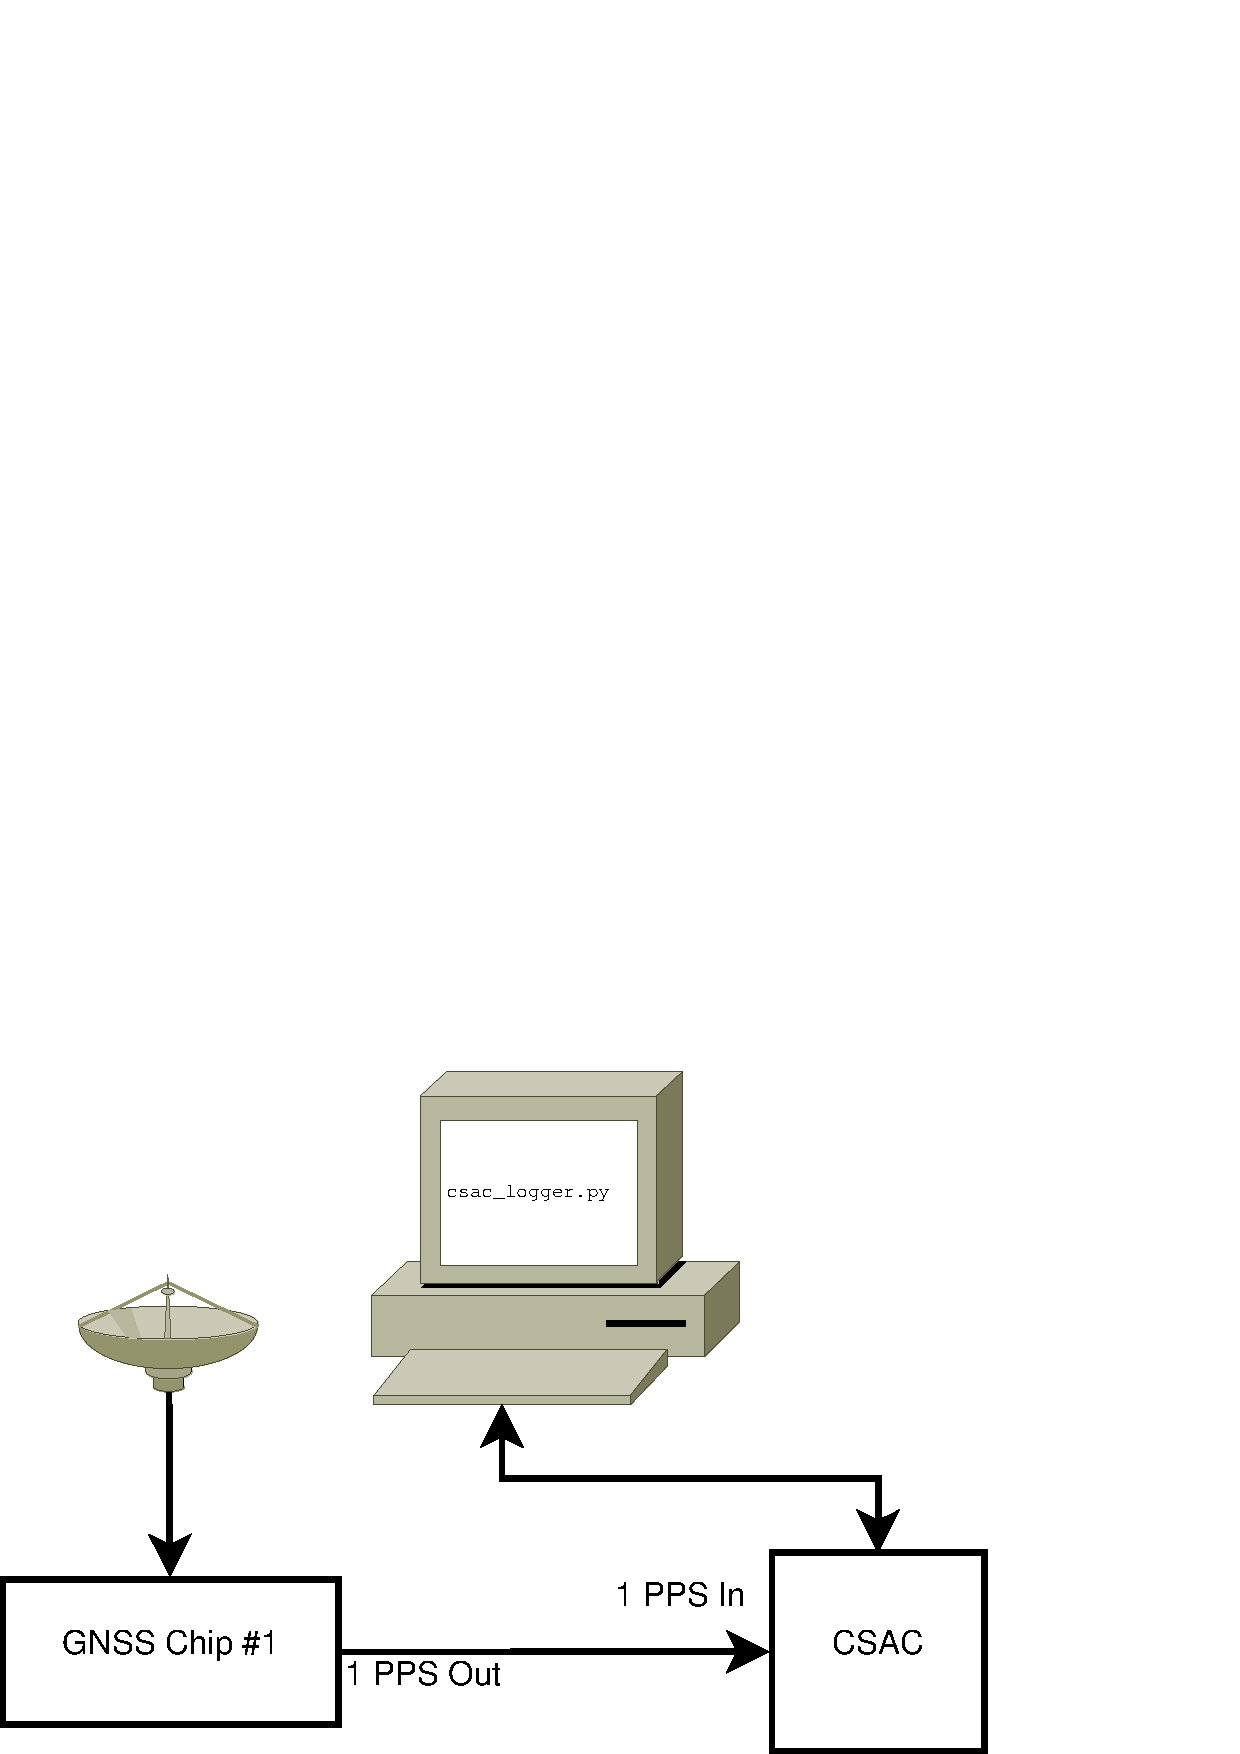
\includegraphics[scale=0.5]{csac_logger.pdf}

\chapter{E-mails}
\section{Correspondence with Mr. Davis}\label{davis_email}
	\begin{Verbatim}[fontsize=\footnotesize ]

Hi Aril,

This would be fine, but you may want to take a look at the Astropy library
and see if their time package would meet your needs. It's certain to be
more robust and well tested. But if you'd like to use my module, please do.
http://docs.astropy.org/en/stable/time/index.html

Best,
Matt Davis

On Sun, Oct 23, 2016 at 2:25 PM Aril Schultzen <aschultzen@gmail.com> wrote:

> Hi!
>
> I am currently writing my master thesis in compsci and I wanted to ask you
> if it was OK if I used your library for converting dates to/from JD and MJD
>   (https://gist.github.com/jiffyclub/1294443) in my implementation? It
> will be used to convert time to MJD for a model and also for stamping logs.
> Your work will of course be acknowledge as your own.
>
> Kind regards
>
> Aril Schultzen
>
	\end{Verbatim}


\end{appendices}